\chapter{Lipid parametrisation} \label{chapter:lip_par}

\lettrine{S}{imulations} of lipids can be a challenging task, especially when the membrane simulated has not been tested experimentally, and thus no comparison can be performed on standard properties such as the area per lipid. Moreover, the parameters describing each lipid species must be carefully chosen, to aim at an accurate reproduction of the natural properties of the membrane.

The work performed in Chapter \ref{chapter:capzip_results} involved the simulation of a mixed membrane which, to our knowledge, has not been experimentally tested. Additionally, one of the lipids involved (DLPG) had not been parametrised before for the GROMOS force field.
%
The procedure of DLPG parametrisation brought to our attention the discrepancy existing between the GROMOS parametrisation of protein and the one employed for lipids, as the two of them are obtained through different procedures: fit to hydration properties for proteins, and quantum mechanics computations for lipids.

The set of lipid parameters derived originally from \citet{Chiu1995} and updated multiple times up to the work of \citet{PogerOrig}, is still regarded as a standard for phosphocholines, and thus used to validate the most recent parametrisation of the force field (GROMOS 54a8 \citep{Reif2012}). However, it does not take into account recent evolutions of the force field, aimed at reparametrising some constitutive moieties which happen to be also part of lipids.
%
For this reason, we performed a reparametrisation of the lipid head group which includes these new descriptions, aiming at an improved consistency with the rest of the force field and monitoring whether they would also improve the agreement with the experimental quantities.

The resulting parametrisation was successful in reproducing key properties such as the area per lipid, and proposed a different interaction with a test peptide with respect to the one outlines by the previous parameter set. Specifically, the new parameters promote a weaker protein-membrane interaction allowing simulations to be less biased from the initial conditions chosen. This is of crucial importance for all simulations in general, and in particular when the sampling is reduced due to computational resources issues.

This chapter consists of the paper ``Lipid Head Group Parameterization for GROMOS 54A8: A Consistent Approach with Protein Force Field Description", published in the \emph{Journal of Chemical Theory and Computation}, together with its Supporting Information. The project was conceived by Prof.\ Franca Fraternali, Dr.\ Christian Margreitter and myself. I carried out all the work, under their guidance; specifically I implemented the new parameter sets, performed and analysed the simulations and selected the best performing parameters to be released. References for the paper and its supplementary material are included separately after each of them (with a numeric notation). All references feature in the bibliography of this thesis as well.

%\includepdf[pages=1-19, nup=1x1, offset = 5mm 0mm, scale = 0.8, pagecommand = \pagestyle{thesis}]{4lip_par/proof.pdf}

%\includepdf[pages=1-6, nup=1x1, offset = 5mm 0mm, scale = 0.8, pagecommand = \pagestyle{thesis}]{4lip_par/Supplementary.pdf}
%\includepdf[pages=7-30, nup=1x2, offset = 5mm 0mm, scale = 0.8, pagecommand = \pagestyle{thesis}, landscape = true]{4lip_par/Supplementary.pdf}
%\includepdf[pages=31-33, nup=1x1, offset = 5mm 0mm, scale = 0.8, pagecommand = \pagestyle{thesis}]{4lip_par/Supplementary.pdf}
%\includepdf[pages=34-37, nup=1x2, offset = 5mm 0mm, scale = 0.8, pagecommand = \pagestyle{thesis}, landscape = true]{4lip_par/Supplementary.pdf}
%\includepdf[pages=38-43, nup=1x1, offset = 5mm 0mm, scale = 0.8, pagecommand = \pagestyle{thesis}]{4lip_par/Supplementary.pdf}
\clearpage

\section{Additional material: effects of membrane undulation}

During the revision process of the paper which constitute this Chapter, it was brought to our attention that membrane undulations might be incompatible with the computation of ApL performed from the sides of the simulation box. The more a membrane patch is deviating from a flat geometry, the more approximate would be such method.
%
Moreover, as the electron density profile is computed as an average over all the $x$ and $y$ positions, undulations of the membrane would result in a broader profile, with more uncertainty on the exact positions of the electron density peaks.

A brief comment on this appears on Section 2.5.1 of the paper, granting that the procedure chosen was suitable for the analysis of the simulations presented, and we would like to provide additional evidence to strengthen the case.
%
This analysis supports as well the choice of using the box sides approach in Chapter \ref{chapter:capzip_results} for simulation without or with low electric field, switching to a computation which takes into account undulations only for the highly curved membranes obtained with a high electric field.

The computation of ApL accounting for the membrane curvature is performed using a Fourier approach according to the work of \citet{Braun2011} and using the software made available from the same publication.
%
This allows to obtain the ratio between the ``true" area per lipid (i.e.\ computed taking into account the undulations of the membrane) and the projected one (i.e.\ from the box sides approach).
%
Figure \ref{fig:apl_und} reports the ratio ApL$_{\text{und}}$/ApL$_{\text{proj}}$ for each lipid and each parameter set: the values span between 1.0020 and 1.0046, which translates into an ApL correction between 0.20 and 0.46\%, or, in absolute value, 0.001-0.003 nm$^2$.
%
These discrepancies are lower than the standard deviation for any of the area per lipid computed, showing that the more accurate computation has no consequence for the purpose of evaluating the ApL and comparing parameter sets.
%
The parameter set showing less discrepancy is Chiu/54a7, compatible with the fact that on average it produces smaller area per lipid: a more packed bilayer results in less freedom for the lipids to undulate.

\begin{figure}[h!]
	\centering
	\includegraphics[width=0.5\textwidth]{4lip_par/pics/apl_localVSbox.pdf}
	\caption[Comparison between methods to compute ApL]{Ratio between area per lipid computed taking into account the undulations of the membrane (according to the procedure devised in \citet{Braun2011}) and the one computed from the projection on the plane parallel to the membrane. A value of 1 would be obtained for a perfectly flat membrane.}
	\label{fig:apl_und}
\end{figure}

Regarding the electron density, to check the influence of the averaging procedure over different locations of the patch, we computed the electron density for the phosphorus atoms on the full patch (256 lipid per leaflet), on a medium patch of roughly one forth in dimension (60 lipids per leaflet, see Figure \ref{fig:patch} for a scheme), and finally a small 12 lipids per leaflet patch. It must be noticed that the GROMACS software, while computing the density perpendicular to the bilayer plane (presently along the $z$ axis), centres the patch analysed around its center of mass, at each time step. This holds for GROMACS versions 5 onward, an version 2016.3 was used for all the analyses presented.

The resulting densities from the three different patches described above are normalised by the number of lipids present in each and compared. Figure \ref{fig:density_patch} shows that the profiles for the full and medium patches are almost identical, while the smaller patch produces narrower peaks.
%
Indeed, computing the full width at half maximum (FWHM) of these peaks, the FWHM of the small patch peaks is 16\% smaller than the FWHM of the large patch peaks.
%
However the distance between phosphorus peaks differ between patches by around 0.1 \AA\ only, showing that the undulations have an effect mainly (or only) on the peaks broadness.
%
As such, the hydrophobic thickness (measured as the distance between the phosphorous peaks) is virtually unvaried, and the difference imputable to the computing procedure is smaller than both the experimental thickness error and the differences arising from the use of different parameter sets.
%
Further analysis must be done on the Luzzati thickness estimate, which depends on the broadness of the water profile. However, it must be noticed that also for this measure, the range of experimental results is quite broad and thus, as for many properties assessed in the paper, likely to be larger than the differences which can derive from the analysis procedure.

\begin{figure}[t!]
\centering
\subbottom[]{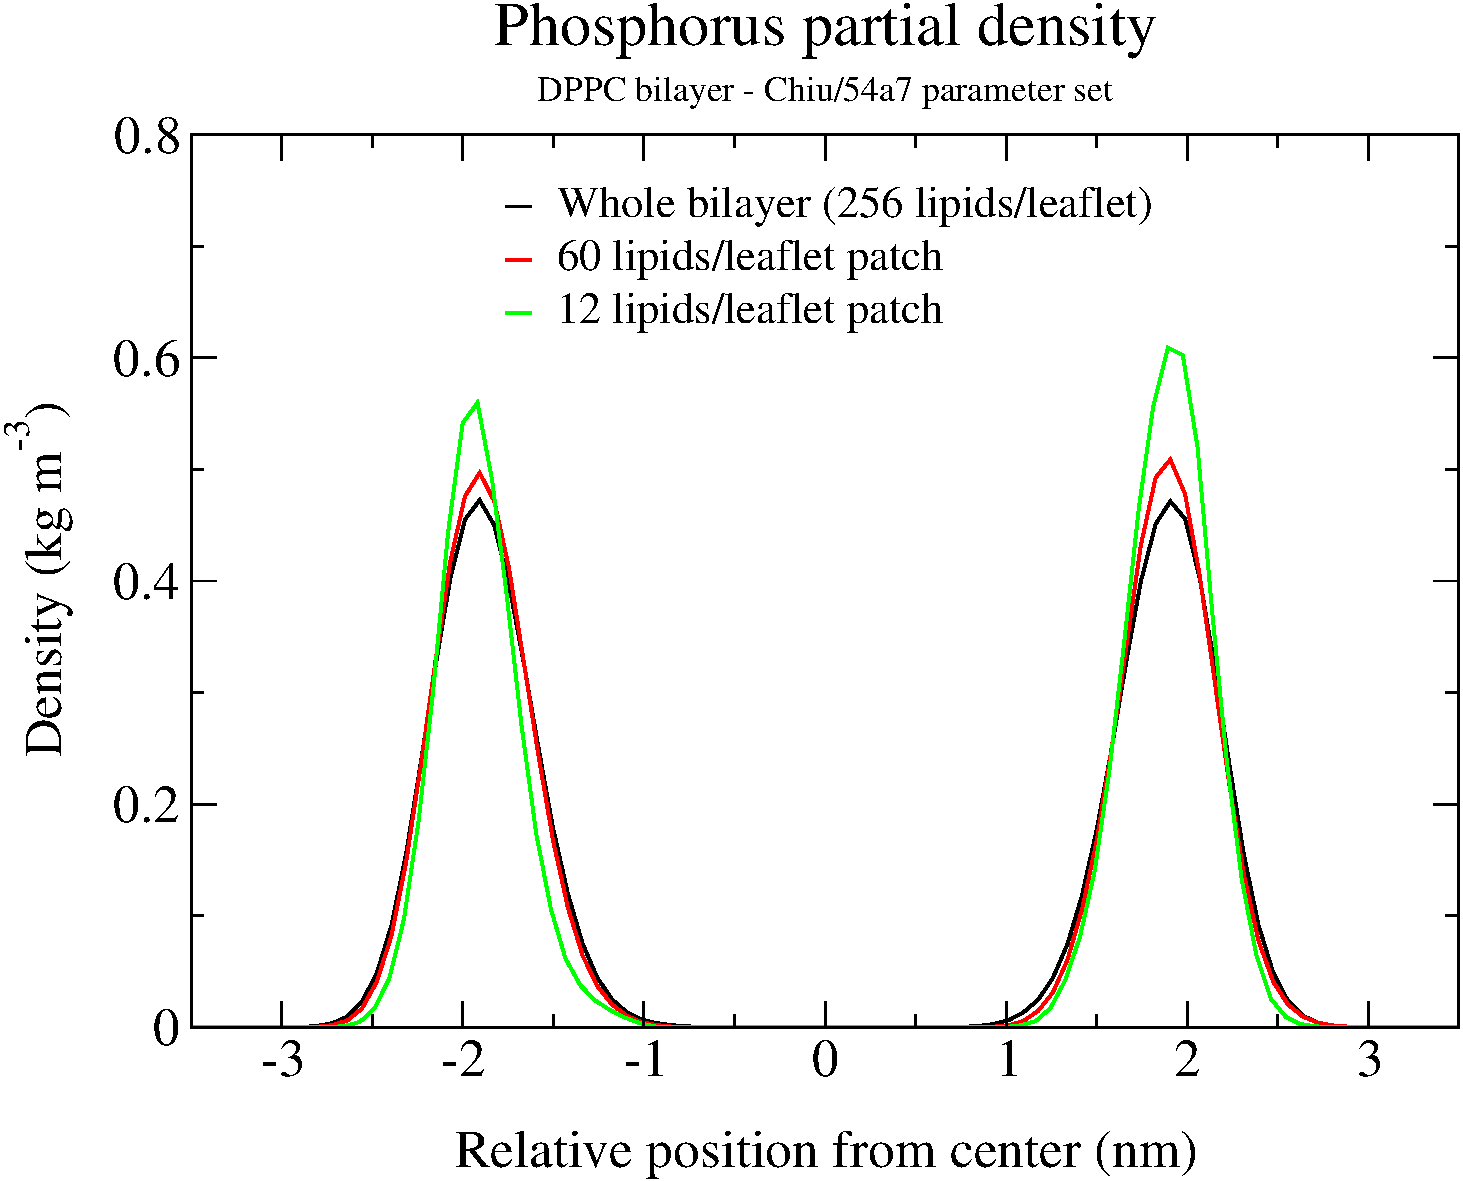
\includegraphics[width=0.55\linewidth, align=c]{4lip_par/pics/compare_density} \label{fig:density_patch}}
\subbottom[]{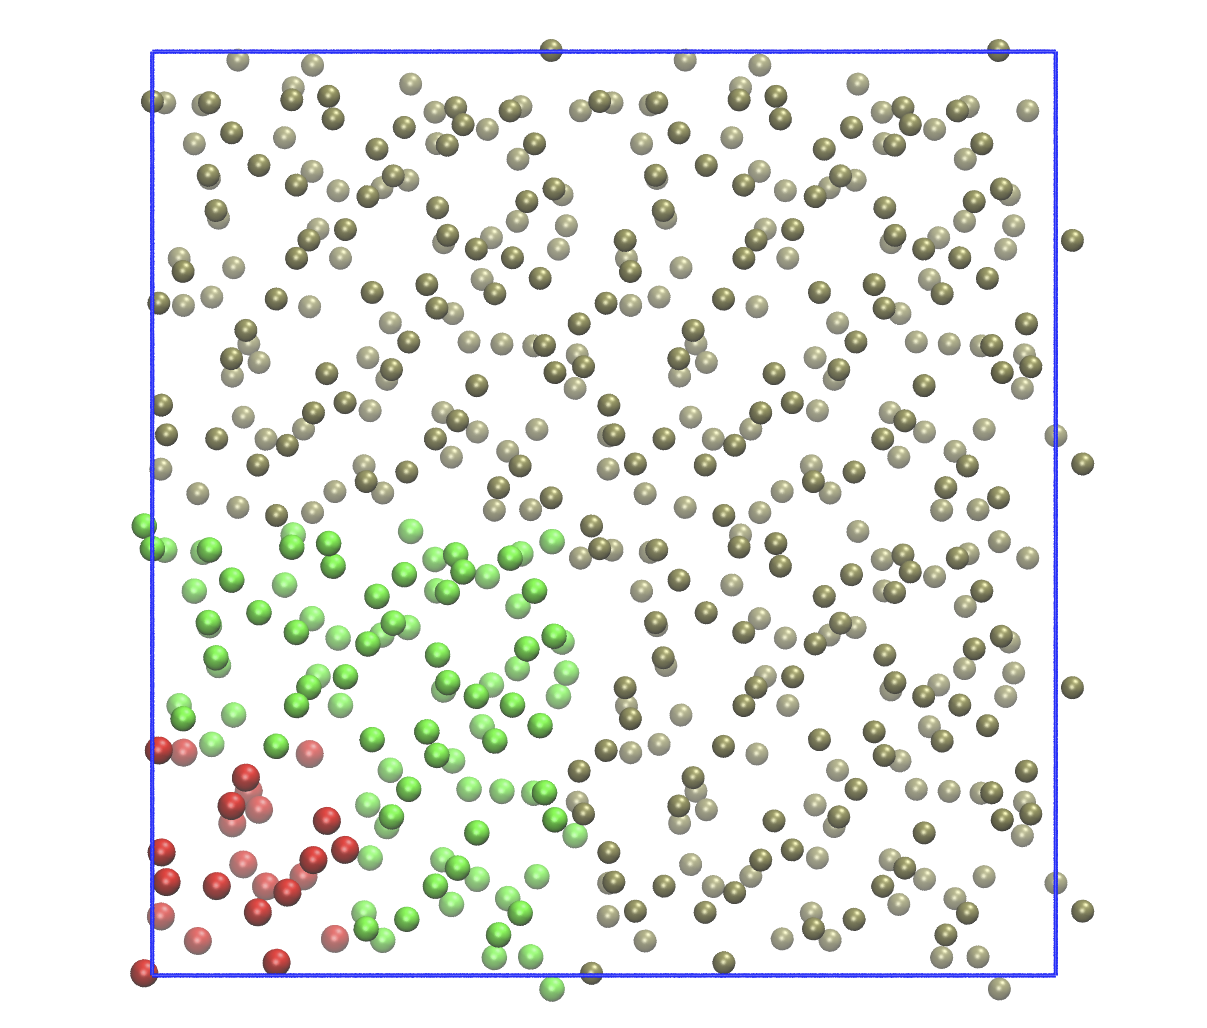
\includegraphics[width=0.35\linewidth, align=c]{4lip_par/pics/patches.png} \label{fig:patch}}
%
\caption[Control computation on bilayer electron density calculation]{(a) Electron density of the phosphorus atom computed on the full membrane, a medium and a small patch. (b) van der Waals representation of the phosphorus atoms of the DPPC lipid bilayer (initial configuration) used for simulations. The simulation box is highlighted in blue. The green plus red regions constitute the medium patch mentioned in the analysis; the red one constitute the small patch.}
\label{fig:density_check}
\end{figure}

\nocite{Abraham2015,Aurenhammer1991,Berendsen1984,Berendsen1995,Berglund2015,Borle1983, Borle1985,Botan2015,Bransden2003,Braun2011,BULDT1978,Castelletto2016,CelineAnezo2003, Chan2006,Chan2007,Chandrasekhar2003,Chandrasekhar2004,Chandrasekhar_vanGunst2001, Chandrasekhar_vanGunst2002,Chiu1995,Chiu2009,Chowdhary2013,Clarke2001,Cocucci2017, Cooper2000,Davis1981,deVries2004,Dickson2014,Ding2015,Doktorova2017,Douliez1995, Douliez1998,doux2012,Einstein1956,Entova2018,Essmann1995,gromacs_man,gromos43a1, Gurtovenko2007flip,Gurtovenko2009,HariLeontiadou2006,Hart2012,Hess1997,Hodder2001, Huang1982,Huang2017,Hwang1998,Jean-Louis2006,Jia2011,Johner2016,Kandasamy2004,
Khalid2015,Klauda2010,Kucerka2011,Kucerka2015,Kukol2009,Lairion2002,Leontiadou2004,
Leontiadou2007,Lewis1987,Lindblom2009,Lipkin2017,Lopes2017,Ma2017,Mabrey1976,Maier2015,
Malkia2004,Margreitter2017,Marinov1996,Marrink2001aggr,Marrink2003,Marrink2005,
McIntosh1986,Miyamoto1992,Mulliken1955,Nagle2000,Nagle2017,Nagle2019,Nguyen2005,
Oostenbrink2004,openStruct,Pan2012,Petrache2000,Petrov2013,Pickar1978,Piggot2011,
Piggot2012,Piggot2017,Pino-Angeles2016,Pluhackova2016,Poger2016,PogerOrig,PogerValid,
Rand1988,Reif2012,Reif2013,Reisser2017,Risselada2008,Schamberger2002,Schibli1999,
Schmid2011,Scott2017,Semchyschyn2004,Sengupta2008,Sharpe2010,Shi2003,Skjevik2015,
Sohlenkamp2016,Starke-Peterkovic2009,Strom2002,Sun1994,Tieleman1998,Tieleman2006flip,
Tironi1995,Ulrich1990,Ulrich1994,Uppulury2015,VanLehn2014a,VanLehn2014b,Venable2017,
Vermeer2007,Vernier2006,Vivcharuk2008,Vogele2018,Wang1994,Wang2006,Wang2012,
Warshaviak2011,Zhang2001,Zhao2000}
